\chapter{Background and Related work}
\label{chap-related}

\section{Background}
\label{sec-cb-background}

\begin{figure}[t]
\begin{center}
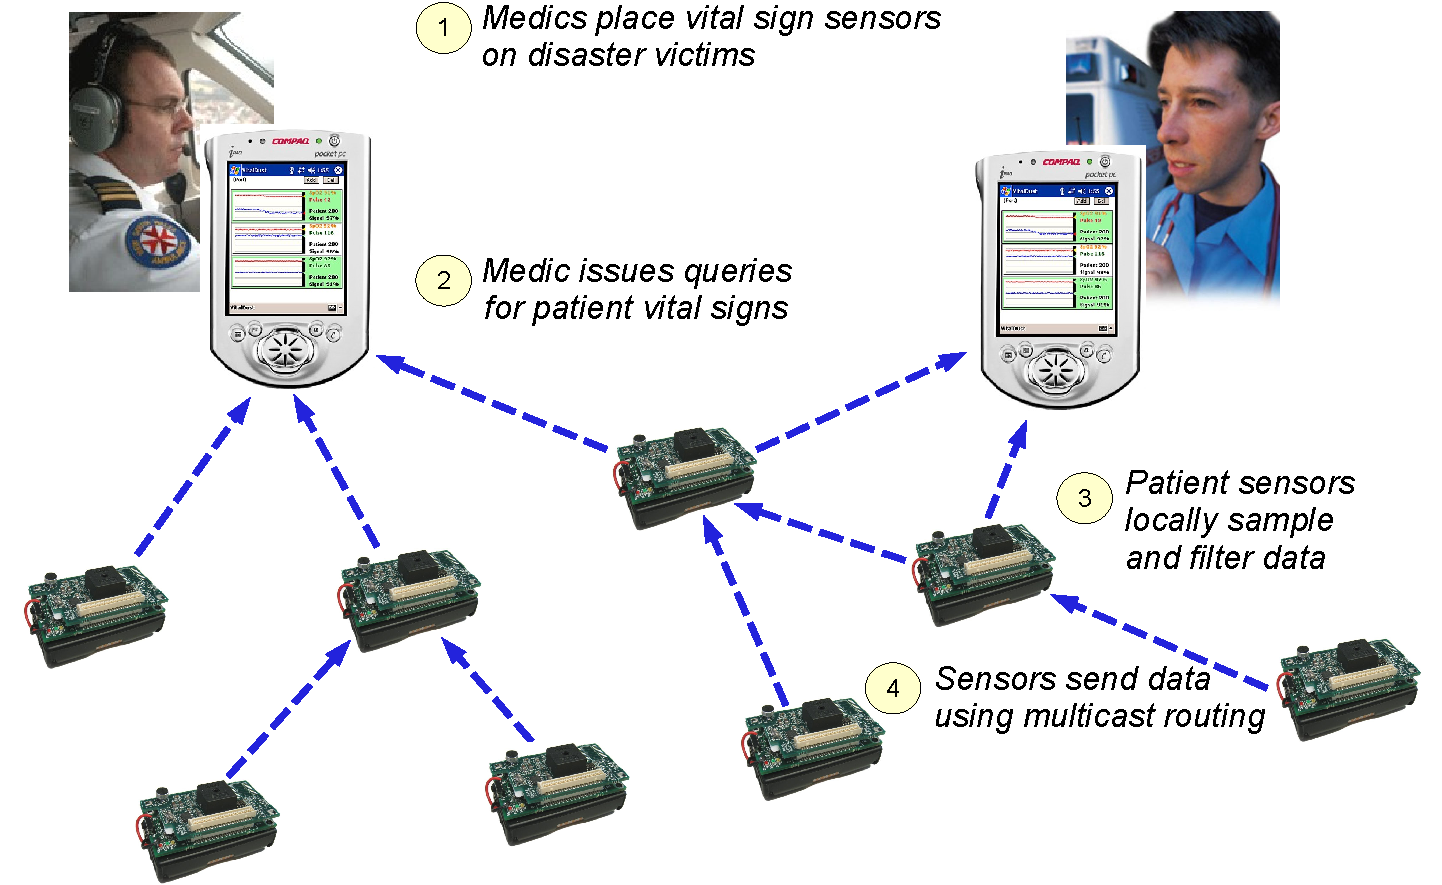
\includegraphics[width=\hsize]{./resources/codeblue-nsdi06/figures/arch/disaster3.pdf} \\
\end{center}
\caption{{\small\bf Use of a medical sensor network in a mass casualty
event.} }
\label{fig-app-example}
\end{figure}


Medical care is an exciting application for sensor networks. The
ability to augment medical telemetry with tiny, wearable, wireless
sensors would have a profound impact on many aspects of clinical
practice. Emergency medical care, triage, and intensive care can all
benefit from continuous vital sign monitoring, especially since it
allows for immediate notification of patient deterioration. Sensor
data can be integrated into electronic patient care records and
retrieved for later analysis. In a wide range of clinical studies,
especially those involving ambulatory or at-home monitoring, wireless
sensors would permit data acquisition at higher resolution and for
longer durations than existing monitoring solutions.

Figure~\ref{fig-app-example} illustrates one application example for
medical sensor networks: monitoring many patients following a
large-scale disaster or mass casualty event, such as a fire or
chemical spill. In this application, each patient is outfitted with
one or more sensors that monitor basic vital signs such as heart rate
or blood oxygen saturation. A limited number of first responders are
responsible for continuously monitoring the patients using handheld
PDAs or other devices.  They receive periodic status updates on each
patient, and can optionally enter other medical information, such as
patient history.  First responders and EMTs perform a wide range of
in-field interventions and assign a triage level to each patient based
on vital signs, history, and resource availability.  Based on
severity, patients may be treated and released in the field or
transported to a hospital or trauma center.

\subsection{Application requirements}

The aforementioned application example motivates the need for a new
software architecture specifically designed for medical applications.
Medical sensor networks differ significantly from more conventional
sensor network designs, which often focus on data collection from large,
spatially distributed networks with low data rates, long lifetime
requirements, and generally a single base
station~\cite{cerpa-habitat,gdi,redwoods,intel-industrial}.  In
contrast, medical sensor networks involve networks of mobile devices
with highly variable data rates and complex communication
patterns. Moreover, periodically recharging batteries is not
problematic in most medical scenarios, as nodes can be readily
serviced by hospital staff.  Table~\ref{table-diffs} outlines these
key differences.

Many of the significant advances in sensor networks, such as routing
protocols~\cite{diffusion,awoo-multihop}, aggregation
techniques~\cite{tinydb-osdi,beyond-average,diffusion}, query
models~\cite{tinydb-sigmod,cougar-sigmodrecord}, and energy-saving
measures~\cite{s-mac,b-mac,sp-sensys05}, should be reevaluated given
these new requirements. Moreover, it is necessary to pull together a
wide range of solutions for device discovery, routing, querying, and
sensor retasking into a complete platform for medical sensor
networks.

\begin{figure}[t]
\begin{center}
\begin{small}
\begin{tabular}{|l|l|l|}  \hline
{\bf Characteristic} & 
{\bf Conventional } &
{\bf Medical apps} \\ 

& {\bf sensor apps} & \\ \hline

{\em Data rate and duty cycle}  & low ($\leq$ 1~Hz) & high (1-1000~Hz) \\
{\em Node population} & fixed, static &  variable, mobile \\
{\em Sensor types} & fixed at deployment & varies over time \\
{\em Data sinks} & single base station & multiple \\
{\em Data aggregation} & extremely beneficial & limited value \\
{\em Node lifetime requirement} & months to years & hours to days \\
{\em Security requirement} &  low & high \\ \hline
\end{tabular}
\end{small}
\end{center}
\caption{{{\small\bf Some important characteristics of medical sensor
networks.}}}
\label{table-diffs}
\end{figure}



\subsection{Existing wireless medical devices}

Wireless medical telemetry is not altogether new. A number of wireless
medical monitors are currently on the market, including
electrocardiographs (EKGs)~\cite{LifeSync,HealthFrontier,apexproch},
pulse oximeters~\cite{nonin,micropaq}, blood pressure
monitors~\cite{cardguard,aanddmedical}, and fetal heart rate and
maternal uterine monitors~\cite{corometrics340m}.  Most of these
devices use Bluetooth or the analog Wireless Medical Telemetry Service
(WMTS) bands~\cite{wmts}, although several employ IEEE 802.11.
However, these systems are generally designed only to ``cut the cord''
between the sensor worn by the patient and a bedside monitor or other
nearby receiving device.  
Few of these devices are designed to be wearable; most remain 
attached to the hospital bed, and those wireless ambulatory products 
on the market are generally large and cumbersome.  



\subsection{Mote-based medical sensor designs}
\label{sec-cb-hardware}

The emergence of low-power, single-chip radios based on the
Bluetooth and 802.15.4~\cite{ieee-802.15.4} standards has precipitated 
the design of small, wearable, truly networked medical sensors. 
The TinyOS mote platforms~\cite{micaz,telos} are small
and lightweight, making them good candidates for prototype medical
sensors, although as we discuss below, smaller form factors and 
better packaging are still needed.

\begin{figure}[t]
\begin{center}
\begin{tabular}{ccc}
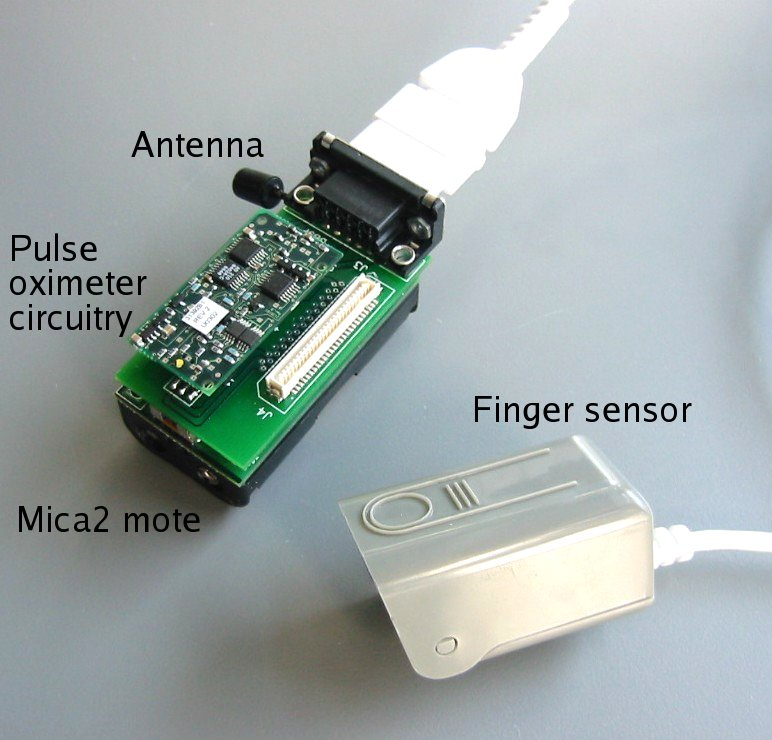
\includegraphics[height=0.18\vsize]{./resources/codeblue-nsdi06/figures/pics/vitaldust3-annotate.jpg}
&
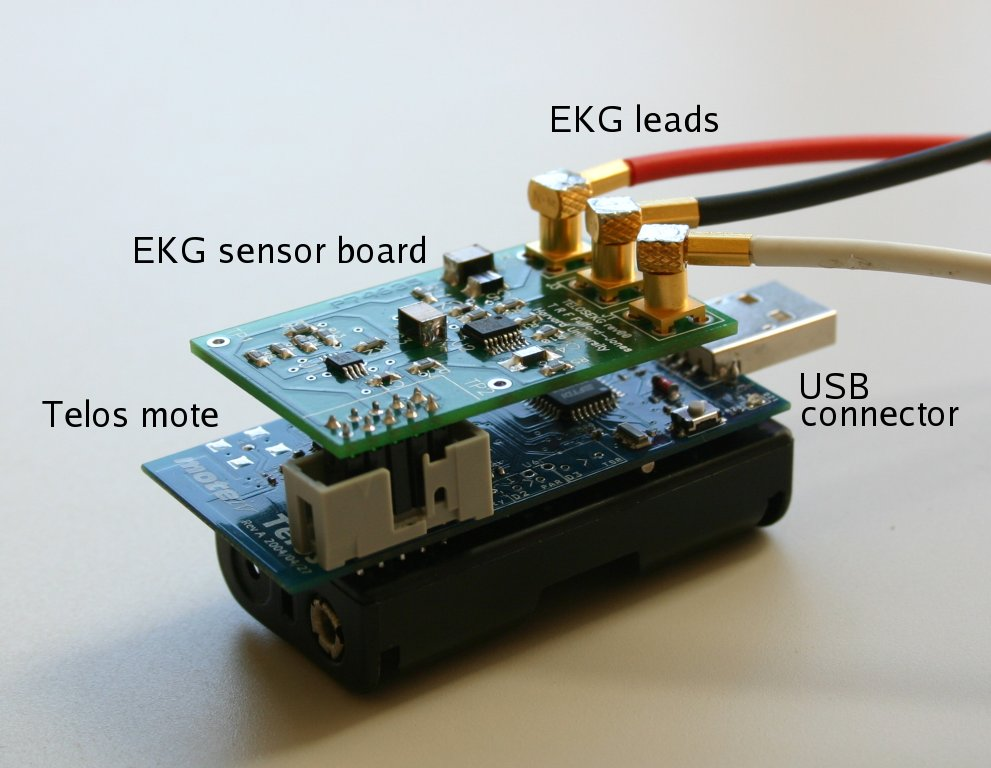
\includegraphics[height=0.18\vsize]{./resources/codeblue-nsdi06/figures/pics/telos-ekg3.jpg} &
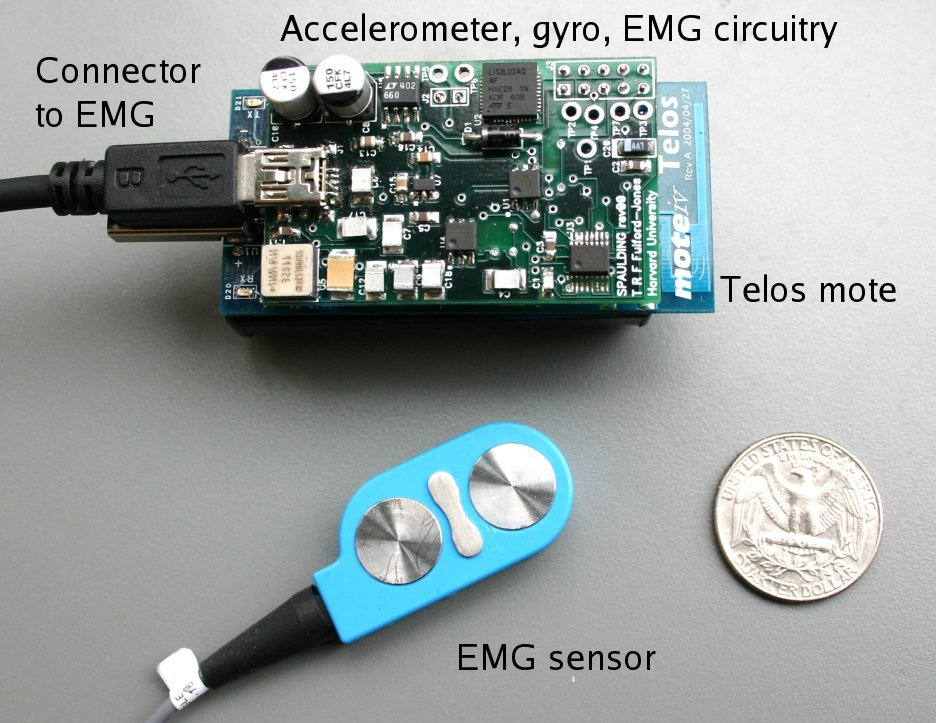
\includegraphics[height=0.18\vsize]{./resources/codeblue-nsdi06/figures/pics/mercury1-annotate-nourl.jpg} \\
{\small\bf (a) Pulse oximeter} & {\small\bf (b) EKG} & {\small\bf (c)
Motion capture and EMG}
\end{tabular}
\end{center}
\caption{{\small {\bf Wireless medical sensors developed by our
group.}}}
\label{fig-sensors}
\end{figure}
To facilitate research into medical sensor networks, 
we have developed a series of wireless medical sensors based
on the Telos~\cite{telos} and MicaZ~\cite{micaz} sensor node
platforms, shown in Figures~\ref{fig-sensors}~and~\ref{fig-pluto}. 
These include the
following:
\begin{description}
\item[Pulse oximeter:] Based on the MicaZ platform, our wireless
pulse oximeter~\cite{codeblue-wames} determines heart rate and blood oxygen 
saturation (SpO$_2$) by measuring the amount of light transmitted through 
a non-invasive finger sensor. It is based on a commercially-available
circuit from BCI, Inc.
\item[Electrocardiograph (EKG):] Based on the Telos platform, our
two-lead EKG~\cite{vitalekg} provides continuous monitoring of the 
electrical activity of the heart, which can be used to diagnose
serious conditions such as arrhythmia or myocardial infarction (heart attack). 
\item[Motion analysis sensor board:] Also based on the Telos, 
this is a specialized suite of sensors for measuring the movement of
body segments, using a three-axis accelerometer and gyroscope. It also
includes an electromyograph (EMG), which measures electrical
impulses of the muscles using a sensor placed on the skin.
It is designed specifically for motion studies in stroke and
Parkinson's Disease patients.
\end{description}

\begin{figure}[t]
\begin{center}
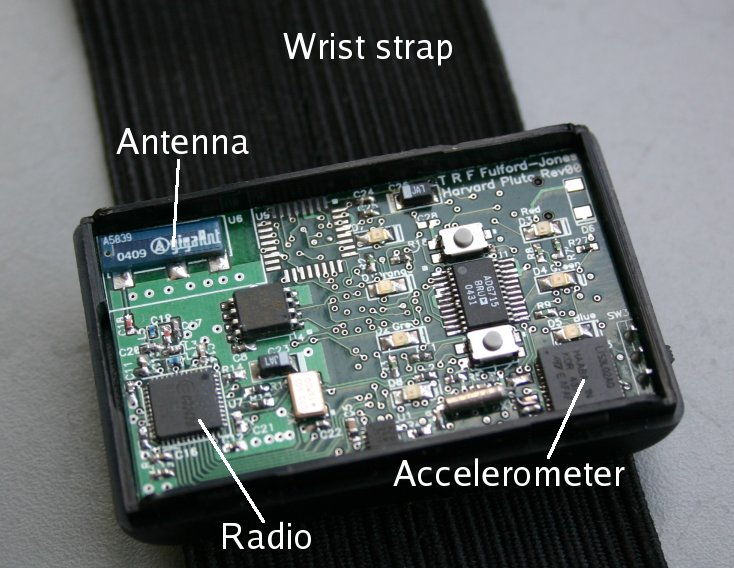
\includegraphics[height=0.18\vsize]{./resources/codeblue-nsdi06/figures/pics/pluto5.jpg} \\
\end{center}
\caption{{\small {\bf The {\em Pluto} custom wearable mote.}}}
\label{fig-pluto}
\end{figure}
Although these sensors are good for experimentation in the lab, their
relatively large size make them less suitable for real medical use. 
To experiment with reduced form factor and increased component
integration, we have developed a custom, miniaturized mote platform,
called {\em Pluto} (Figure~\ref{fig-pluto}). Pluto measures 
57~$\times$~36~$\times$~16~mm and incorporates a 
TI MSP430 processor, a Chipcon CC2420 radio, a thin, rechargeable 
Li-polymer battery, a surface-mount antenna, and a three-axis 
accelerometer. No software changes are required to run TinyOS
applications on Pluto, since it is compatible with the popular Telos
mote platform. 


\section{Wireless patient monitoring systems}
A number of other research projects are exploring medical sensor 
networks. Many of these are concerned with developing
wearable medical sensors~\cite{bennylo-05,bsn-node,eugene-shih-demo}, 
while others have developed infrastructures for monitoring 
individual patients during daily activity~\cite{mobihealth-ist},
at home~\cite{proactive-health}, or at a hospital~\cite{ubimon}.
In contrast, our focus is to develop a robust, scalable infrastructure 
for deploying sensor networks in a range of medical settings.

More closely related to our efforts are systems for enabling large
numbers of medical sensors to be used for disaster response. The
SMART~\cite{smart}, AID-N~\cite{aid-n}, and WiiSARD~\cite{wiisard}
teams are among several funded through a US National Library of
Medicine effort to develop new technologies for disaster management.
The AID-N group is making use of our sensor designs and CodeBlue architecture, and the SMART
team has developed a mote-based EKG~\cite{eugene-shih-demo} that is
largely equivalent to our design described in
Section~\ref{sec-cb-hardware}.  The WiiSARD group has developed a
prototype pulse oximeter based on an 802.11-equipped PDA, but its size
and power requirements make it impractical for real use. The
WiiSARD and SMART designs call for a central server to collect and
distribute all sensor data, an approach which benefits from simplicity
but has obvious reliability and scalability considerations. 

MEDiSN~\cite{medisn-bodynets09}, a highly related research project, 
focuses on monitoring patients in hospital emergency departments. Leveraging
the hospital environment, the system architecture contains two types of sensor
nodes: physiological monitors and relay points. Physiological monitors are
battery powered mobile motes that are attached to patients and perform only
sampling of physiological signals.  Relay points are, on the other hand,
wall-powered static motes that can be located strategically to form a high
quality collection routing tree rooted at a single base station. Relay points
are only responsible for routing data packets back to the base station. The
MEDiSN system simplifies the software for physiological monitors due to the
separation of responsibility of sampling and routing. At the same time, such
advantage also limits the usage of the system because it requires the
infrastructure support from the hospital environment.

AlarmNet~\cite{alarmnet-network08} is another project that aims to use sensor
networks to improve medical care. This project focuses on long-term monitoring
using both wearable and infrastructure supported sensors in order to provide
an intelligent assisted living environment. The AlarmNet system makes use of
body area networks to perform on-body physiological sensing and activity
classification. In the environment, such as the patient's home or a hospital
room, there are {\em emplaced sensors} that collects data such as temperature,
dust, light or perform motion detection. The data from the patient body
sensors are sent through the emplaced sensors, i.e. wall powered static nodes,
that are responsible for routing the data to a back-end database server. Because
the goal of the system focuses on assisting long-term care in a home or
hospital setting, it is not applicable to more ad-hoc scenarios such as 
disaster response.


\section{Routing in Sensor Networks}

Much work on routing protocols in sensor networks has focused
on forming stable routes to a single aggregation point, i.e. a base
station. Many approaches have been proposed for spanning-tree formation,
parent selection, and hop-by-hop data aggregation as data flows up the
tree~\cite{awoo-multihop,dimensions,tinydb-osdi,nath-synopsis-diffusion}.
These protocols are appropriate for networks consisting
of stationary nodes that are primarily focused on data
collection. However, several emerging applications for sensor
networks require more general topologies as well as
communication with mobile nodes. 
Examples include tracking firefighters in a burning
building~\cite{paul-wright-firefighter}, data collection with mobile
sensors~\cite{nims,kansal-mobisys04,zebranet-mobisys04},
and monitoring the location and health status of disaster
victims~\cite{codeblue-ieeepc}.

The mobile ad-hoc networking (MANET) community has developed a wide range
of protocols for unicast and multicast routing using mobile wireless
devices~\cite{aodv,admr,dsr,dsdv}. 
Many of these protocols have been studied only under simulation 
using simplistic radio models, and do not consider issues such as bandwidth
or memory limitations. In contrast, the sensor network community has 
demanded solutions that work on real hardware with limited resources.
As a result, much of the MANET work has been overlooked by the sensor
network community in favor of specially-tailored protocols that focus
on energy management~\cite{stem,leach}, 
reliability~\cite{awoo-multihop,psfq,esrt}, and in-network
aggregation~\cite{tinydb-osdi,nath-synopsis-diffusion}.

Our goal is to bridge the gap between the mobile ad-hoc networking
field and the state-of-the-art in sensor networks. 
By doing so, we hope to tap into the rich body of work in the MANET
community, which may require reevaluating and redesigning these 
protocols as necessary. In particular, we identify several challenges
to implementing MANET-based protocols on sensor nodes. The
limited memory, computational power, and radio bandwidth deeply impact
the implementation strategy. 
For example, high protocol overheads and
large routing tables are infeasible with popular sensor mote platforms.
In addition, the realities of radio propagation, such as lossy and 
asymmetric links, require careful evaluation of path selection metrics.

\subsection{MANET routing protocols}

Researchers in the MANET community have put in a great deal of effort into
the design of routing protocols for ad-hoc networks. For unicast use, 
DSDV~\cite{dsdv}, AODV~\cite{aodv} and DSR~\cite{dsr} are 
three of the most commonly-studied routing protocols for MANET 
applications. DSDV is a proactive distance-vector based routing 
protocol. It maintains a routing table containing shortest hop 
counts from a node to every other node in the network. The table 
is built up by periodically exchanging routing tables among 
neighbors. With DSDV, every possible route in the network is maintained 
by the protocol. AODV is also based on distance-vector but it works 
on-demand rather than proactively. A flood of route request 
message is sent out whenever a node needs to find a route. The 
destination replies with a route reply packet following the 
reverse path of the route request message. DSR is another popular
on-demand unicast protocol that discovers routes in a similar
fashion as AODV. However, in DSR, nodes don't keep the states
of next hop information. Rather, source nodes are in charge of specifying
the entire route in every data packet they want to send out.

A wide range of ad-hoc multicast routing protocols have also been 
proposed.  We only describe three representative ones here: ADMR~\cite{admr},
ODMRP~\cite{odmrp} and MAODV~\cite{maodv} by comparing the route establishment
and route maintenance mechanisms.
The major differences between ODMRP and ADMR are in the
tree-pruning mechanisms and how broken links are repaired. 
ODMRP prunes the forwarders
based on a lifetime value associated with each forwarding state.
The lifetime is decreased every time a timer fires and is reset
every time the node is re-selected as a forwarder. This is 
basically equivalent to the active reinforcement technique
implemented in TinyADMR, as described in Chapter~\ref{chap-tinyadmr}. ADMR only reinforces forwarders based on 
passive acknowledgments. ODMRP contains a mobility
prediction scheme that acquires the information about the movement 
of a node using GPS-derived location information. 
Based on a fixed-range radio model, it predicts when two nodes 
will be out of communication range and adapts the re-discovery timer accordingly. 

In MAODV, route discovery also begins with network flooding.
However, MAODV does not differentiate data senders from 
receivers in the multicast tree. All nodes which are already in a 
multicast group will answer the discovery message with a unicast
packet following the reverse paths of the discovery messages. 
The node that sent out the discovery message then picks the best
route to connect to the tree according to the multiple reply
messages it has received. To detect link failures, MAODV requires
every node to broadcast a {\em hello} message periodically. If a node
stops receiving {\em hello} messages from a particular node, it will
initiate the route repair process.


Although the above mentioned MANET multicast protocols 
were all carefully designed, all of them have been evaluated 
only through simulations with simple radio models.
The simulations often ignore link asymmetry and assume a fixed 
communication range.


\subsection{Studies of real-world link quality }

Studies of link-level data delivery characteristics of wireless 
networks have confirmed that the assumption of fixed-range, symmetric
links is unrealistic~\cite{connectivity-sigcomm04,
scale, ganesan-empirical}. New routing metrics based on 
dynamic link quality estimation~\cite{etx,awoo-multihop} have been
proposed to alleviate this problem by selecting longer but more 
reliable routes.

Unfortunately, the MANET routing protocols described above all adopt hop 
count as the path routing metric.  
This implies that the protocol may favor shorter paths
over longer paths with higher reliability. 
Therefore, it is unclear from the current literature 
how well the proposed MANET multicast routing protocols will work 
if they are deployed in a real environment using real radio 
communication channels.

\subsection{Routing in TinyOS-based sensor networks}

Studies of routing in sensor networks have primarily been focused on 
building a single spanning tree that routes messages from all the 
nodes in the network to a single base 
station~\cite{awoo-multihop,dimensions,tinydb-osdi,nath-synopsis-diffusion,diffusion}.
Such a global spanning tree is useful for a range of sensor
network applications that involve network-wide data 
collection~\cite{gdi, habitat-cacm, countersniper-sensys04}.  

Woo et al.~\cite{awoo-multihop} carefully studied design
strategies for many-to-one spanning trees in sensor networks.
They found maintaining a spanning tree with highly-reliable links
is non-trivial and requires dynamic link estimation on each sensor node.
The dynamic link estimation proposed in their work is performed by
passively snooping packets from other nodes and using a window mean
EWMA to estimate link quality over time. 
Their evaluation is based on a simulation model derived from 
measurements of link quality between two nodes placed at increasing 
distances. This work also highlights several eviction policies for 
neighbor tables on each node.

\subsubsection{TinyOS implementation of MANET protocols}

Because TinyOS-based sensor networks are still relatively young
in comparison to the vast body of literature on MANET protocols,
we have been unable to identify many TinyOS-based implementations
of MANET protocols. We are only aware of the TinyOS implementations 
of DSDV and AODV by Yarvis et al.~\cite{yarvis, tinyaodv}. 
Among the two protocols, only DSDV was studied and published. 
In ~\cite{yarvis}, the authors present results for an implementation
of DSDV, and the authors also point out that selecting
high-quality links outperforms shortest-hop-count paths.

\section{Sensor network query systems}

TinyDB~\cite{tinydb-osdi}, Cougar~\cite{cougar-sigmodrecord}, and
Directed Diffusion~\cite{diffusion} are three well-known querying
schemes for sensor network applications. Cougar and TinyDB both
provide an SQL-like interface for querying a sensor network.  They
focus on collecting data at a single base station and emphasize
optimization through in-network aggregation, which is inappropriate
for medical applications.  Directed Diffusion defines queries as a set
of attribute-value pairs, and is conceptually flexible enough to
support most of the needs of CodeBlue.  However, the diffusion model
also emphasizes in-network aggregation and data centric routing.  This
is appropriate when the query is conceptually to the {\em entire
network}, but is less suited in our domain, where we are concerned
with data from a {\em particular} patient. Thus, in CodeBlue, we chose to 
separate the query processor from routing layer and design each with the
specific target of medical applications in mind.

\section{Debugging and monitoring of sensor networks}
\label{sec-livenet-background}

Sensor networks are becoming increasingly complex, and correct
behavior often involves subtle interactions between the link layer, 
routing protocol, and application logic. Achieving a deep
understanding of network dynamics is extremely challenging for 
real sensor network deployments. It is often important to study a
sensor deployment {\em in situ}, that is, in its ``natural'' setting
(rather than as part of a testbed or simulation), as well as in
situations where it is impossible or undesirable to add additional
instrumentation. These requirements suggest 
the need for {\em passive} and {\em external} observation of
sensor network behavior.

The most common approach to sensor network development is 
simulation~\cite{tossim,ptossim,avrora}, which provides 
an easy means for instrumenting code and observing the global
behavior of the (simulated) application. 
However, the behavior of a deployed network 
may vary substantially from simulation results. Although simulation
is an invaluable development and debugging tool, no simulator can
perfectly capture the environment, radio channel characteristics,
variations in hardware calibration, and other effects that are so
vexing for real world deployments.

Sensor network testbeds~\cite{mirage,motelab,emstar,emulab} provide a
more realistic debugging environment. However, testbeds are generally
deployed in controlled settings (such as office buildings or
laboratories) and make use of wired back-channels for powering, 
programming, and communicating with individual nodes. In fielded
sensor networks, however, such an approach is clearly impractical.
This problem is compounded in applications involving mobile sensor
nodes.


\subsection{Sensor network debugging tools}
Several previous systems focus on monitoring
and debugging live sensor deployments. Sympathy~\cite{sympathy} is a
system for reasoning about sensor node failures using information 
collected at {\em sink nodes} in the network. Sympathy has two
fundamental limitations that we believe limit its applicability.
First, Sympathy requires that the sensor node software be instrumented 
to transmit periodic {\em metrics} back to the sink node. 
In many cases, it is often
impossible or undesirable to introduce additional instrumentation
into a live deployment. It may not be possible to reprogram sensor
nodes following a deployment (especially if the nodes are closed or
provided by a third party), and instrumentation can change the 
behavior of the network in subtle ways. Second, Sympathy is limited to 
observe network state at sink nodes which may be multiple routing hops 
from the sensor nodes in question. As a result, errant behavior 
deep in the routing tree may not be observed by the sink. 

SNMS~\cite{snms-ewsn05} and Memento~\cite{rost2006memento} are two 
management tools designed for inspecting state in live sensor 
networks. They perform functions such as neighborhood tracking,
failure detection, and reporting inconsistent routing state.
Like Sympathy, these systems involve adding code to the sensor
network application. Both systems attempt to minimize the 
amount of information they transmit to limit bandwidth and energy consumption.
EnviroLog~\cite{envirolog} is a logging tool that is compiled into 
sensor network applications. It records function call traces to the
node's flash. After deployment, EnviroLog can replay the call trace 
to replicate node behavior.

\subsection{Passive monitoring tools}
Jigsaw~\cite{jigsaw} and Wit~\cite{wit} are both passive monitoring tools
designed for IEEE 802.11 wireless networks. Our ideas in passive monitoring
were largely inspired by Jigsaw and Wit. In
these systems, multiple sniffer nodes collect packet traces, which
are then merged into a single trace representing the network's global
behavior. A series of analyses can then be performed on the global
trace, for example, understanding the behavior of the 802.11 CSMA
algorithm under varying loads, or performance artifacts due to
co-channel interference. 

Several other projects have leveraged passive monitoring for studying
802.11 networks. Jigsaw and Wit build upon earlier work by Yeo
{\em et al.}~\cite{yeo-wise04} for trace merging.
Jardosh {\em et al.}~\cite{jardosh-congestion} and Rodrig {\em et
al.}~\cite{rodrig-sigcomm05} describe trace-based analysis of 802.11
behavior in congested settings.


SNIF~\cite{snif-demo-ewsn07} is another passive monitoring system specifically
designed for sensor networks. 
SNIF is focused primarily on debugging
the causes of failures in sensor networks. SNIF uses sniffers that transmit
complete packet traces to a base station via a Bluetooth scatternet.
Apart from the scalability limitations of the scatternet itself,
interference between Bluetooth and 802.15.4~radios commonly used by
sensor networks is a concern, potentially causing the monitoring
infrastructure to interfere with the network's
operation. 

\section{Summary}

In this chapter, we have defined the application requirements of medical sensor
networks, introduced our target hardware platform, and surveyed related work
on wireless patient monitoring systems, sensor network query model, ad-hoc
routing protocols, and passive monitoring approaches for wireless networks.
The requirements for medical sensor networks are different from conventional
sensor network systems because medical sensor networks involve mobile nodes,
variable data rate, multiple sinks and multiple dynamic traffic flows. Earlier
wireless patient monitoring systems typically are not concerned with
resource constraints and often assume IEEE 802.11 or other existing networking
infrastructure available in hospitals or home settings. 

Existing sensor network query models are not
adequate for medical sensor networks because they are designed to collect data
from the entire network and usually couple query and routing layers.
Therefore, these query systems can not leverage features provided by general
purpose routing protocols. Several ad-hoc routing protocols provide the
multicast capability for CodeBlue, but they are not concerned about resource
limitations and have not been tested in realistic radio environments. 
We also surveyed the techniques for debugging and monitoring sensor networks.
Many current approaches are not adequate because they either involve intrusive code
instrumentation, require node storage space, potentially interfere with the
monitored network, or only focus on low level dynamics of IEEE 802.11 networks. 

Starting from these existing systems and techniques surveyed in this chapter,
our goal in this dissertation research is to provide the missing pieces for
building medical sensor networks on resource limited sensor nodes. In the
following chapters of this dissertation, we address the challenges highlighted
in this chapter and Chapter~\ref{chap-intro} by designing and evaluating the
CodeBlue medical sensor network architecture, TinyADMR multicast routing
layer, and LiveNet passive monitoring system.
